\chapter{\hobbit{} block set overview} \label{apx:BlockOverview}
The blocks of \toolname{}' toolbox are divided in the following categories:

\begin{itemize}
    \item Custom Blocks: all blocks which are created with the block configuraton interface (\prettyref{sec:BlockConfiguration})
    \item Move: blocks to move \hobbit{}
    \item Arm Control: blocks, which allows to move \hobbit{}'s arm
    \item Interaction: any form of blocks, which allows \hobbit{} to communicate with the user
    \item Logic: collection of Blockly's predefined logic blocks
    \item Loop: collection of Blockly's predefined looping blocks
    \item Math: collection of Blockly's predefined math blocks
    \item Text: collection of Blockly's predefined text blocks
    \item Lists: collection of Blockly's predefined list blocks
    \item Variables: a category to create and use variables
    \item Functions: a category to create and use functions
\end{itemize}

This section contains an overview of all blocks created for \hobbit{}'s interface, a description of Blockly's predefined blocks can be found in \cite{BlocklyBlockWiki}.

\begin{center}
    \begin{tabular} {c|c}
        \hline
        Block & Description \\ \hline
        \raisebox{-\totalheight}{
\includegraphics[width=0.3\textwidth]{graphics/blocks/undock.png}} & Undock \hobbit{} from charger \\ \hline
        \raisebox{-\totalheight}{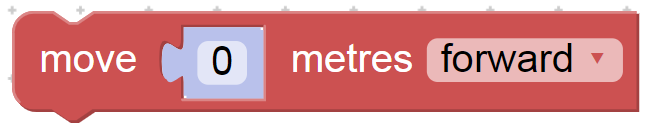
\includegraphics[width=0.3\textwidth]{graphics/blocks/move.png}} & Move \hobbit{} in the given direction \\ \hline
        \raisebox{-\totalheight}{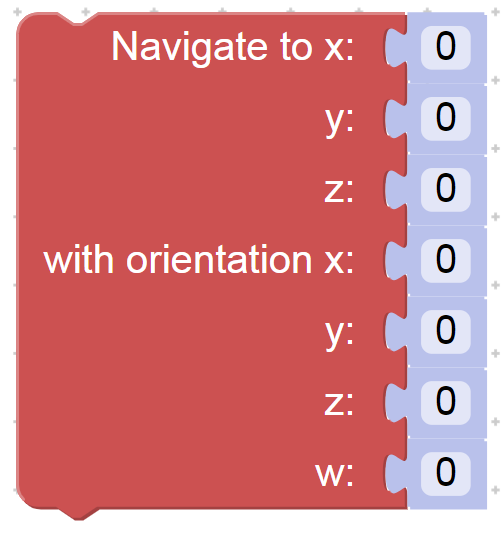
\includegraphics[width=0.3\textwidth]{graphics/blocks/navigation.png}} & Navigate to given pose \\ \hline
        \raisebox{-\totalheight}{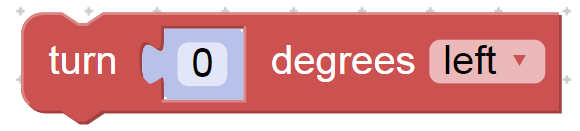
\includegraphics[width=0.3\textwidth]{graphics/blocks/turn.png}} & Rotate \hobbit{} in the given direction \\ \hline
        \raisebox{-\totalheight}{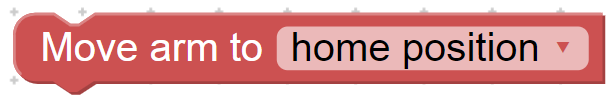
\includegraphics[width=0.3\textwidth]{graphics/blocks/moveArm.png}} & Move \hobbit{}'s arm to the given position \\ \hline
        \raisebox{-\totalheight}{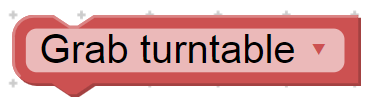
\includegraphics[width=0.3\textwidth]{graphics/blocks/turntable.png}} & Perform the given action with the turntable \\ \hline
        \raisebox{-\totalheight}{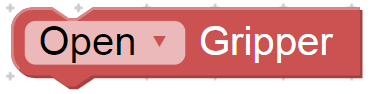
\includegraphics[width=0.3\textwidth]{graphics/blocks/gripper.png}} & Open or close the gripper \\ \hline
        \raisebox{-\totalheight}{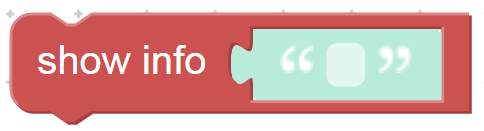
\includegraphics[width=0.3\textwidth]{graphics/blocks/info.png}} & Show an info on \hobbit{}'s tablet \\ \hline
        \raisebox{-\totalheight}{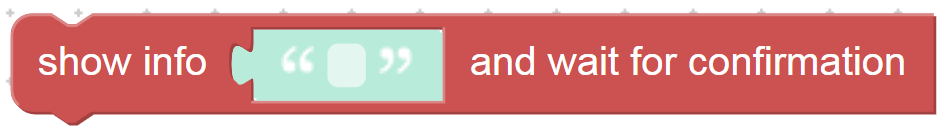
\includegraphics[width=0.3\textwidth]{graphics/blocks/confirm.png}} & Show an info on \hobbit{}'s tablet and wait for confirmation \\ \hline
        \raisebox{-\totalheight}{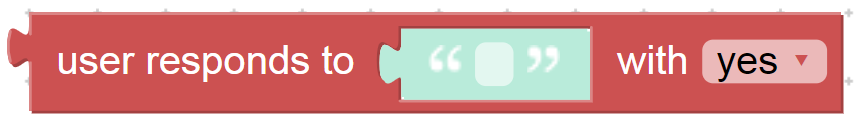
\includegraphics[width=0.3\textwidth]{graphics/blocks/yesno.png}} & Get user's answer to a yes–no question \\ \hline
        \raisebox{-\totalheight}{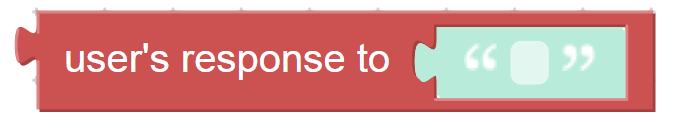
\includegraphics[width=0.3\textwidth]{graphics/blocks/question.png}} & Display the given question on \hobbit{}'s tablet and get user's answer \\ \hline
        \raisebox{-\totalheight}{
\includegraphics[width=0.3\textwidth]{graphics/blocks/headmove.png}} & Move \hobbit{}'s head to the given position \\ \hline
        \raisebox{-\totalheight}{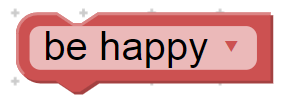
\includegraphics[width=0.3\textwidth]{graphics/blocks/emotion.png}} & Set \hobbit{}'s eyes according to the given emotion \\ \hline
    \end{tabular}
\end{center}